%!TEX root = ../thesis.tex
\section{OVERVIEW}

This section is devoted to the description of the available geo-spatial data analysis tools. Also,
modern web-based maps libraries are considered. Finally, data formats used for storing geographical
data are reviewed.

\subsection{Geographical Analysis Software}

There are many tools available for analysis of the geo-spatial data. However, in this section
three different tools such as GRASS, QGIS, CartoDB will be reviewed. Although, mentioned
tools may be considered as GIS, each of them provides different functionality and oriented
on different user audience.

\subsubsection{GRASS GIS}

\begin{figure}[ht]
  {\par\centering
  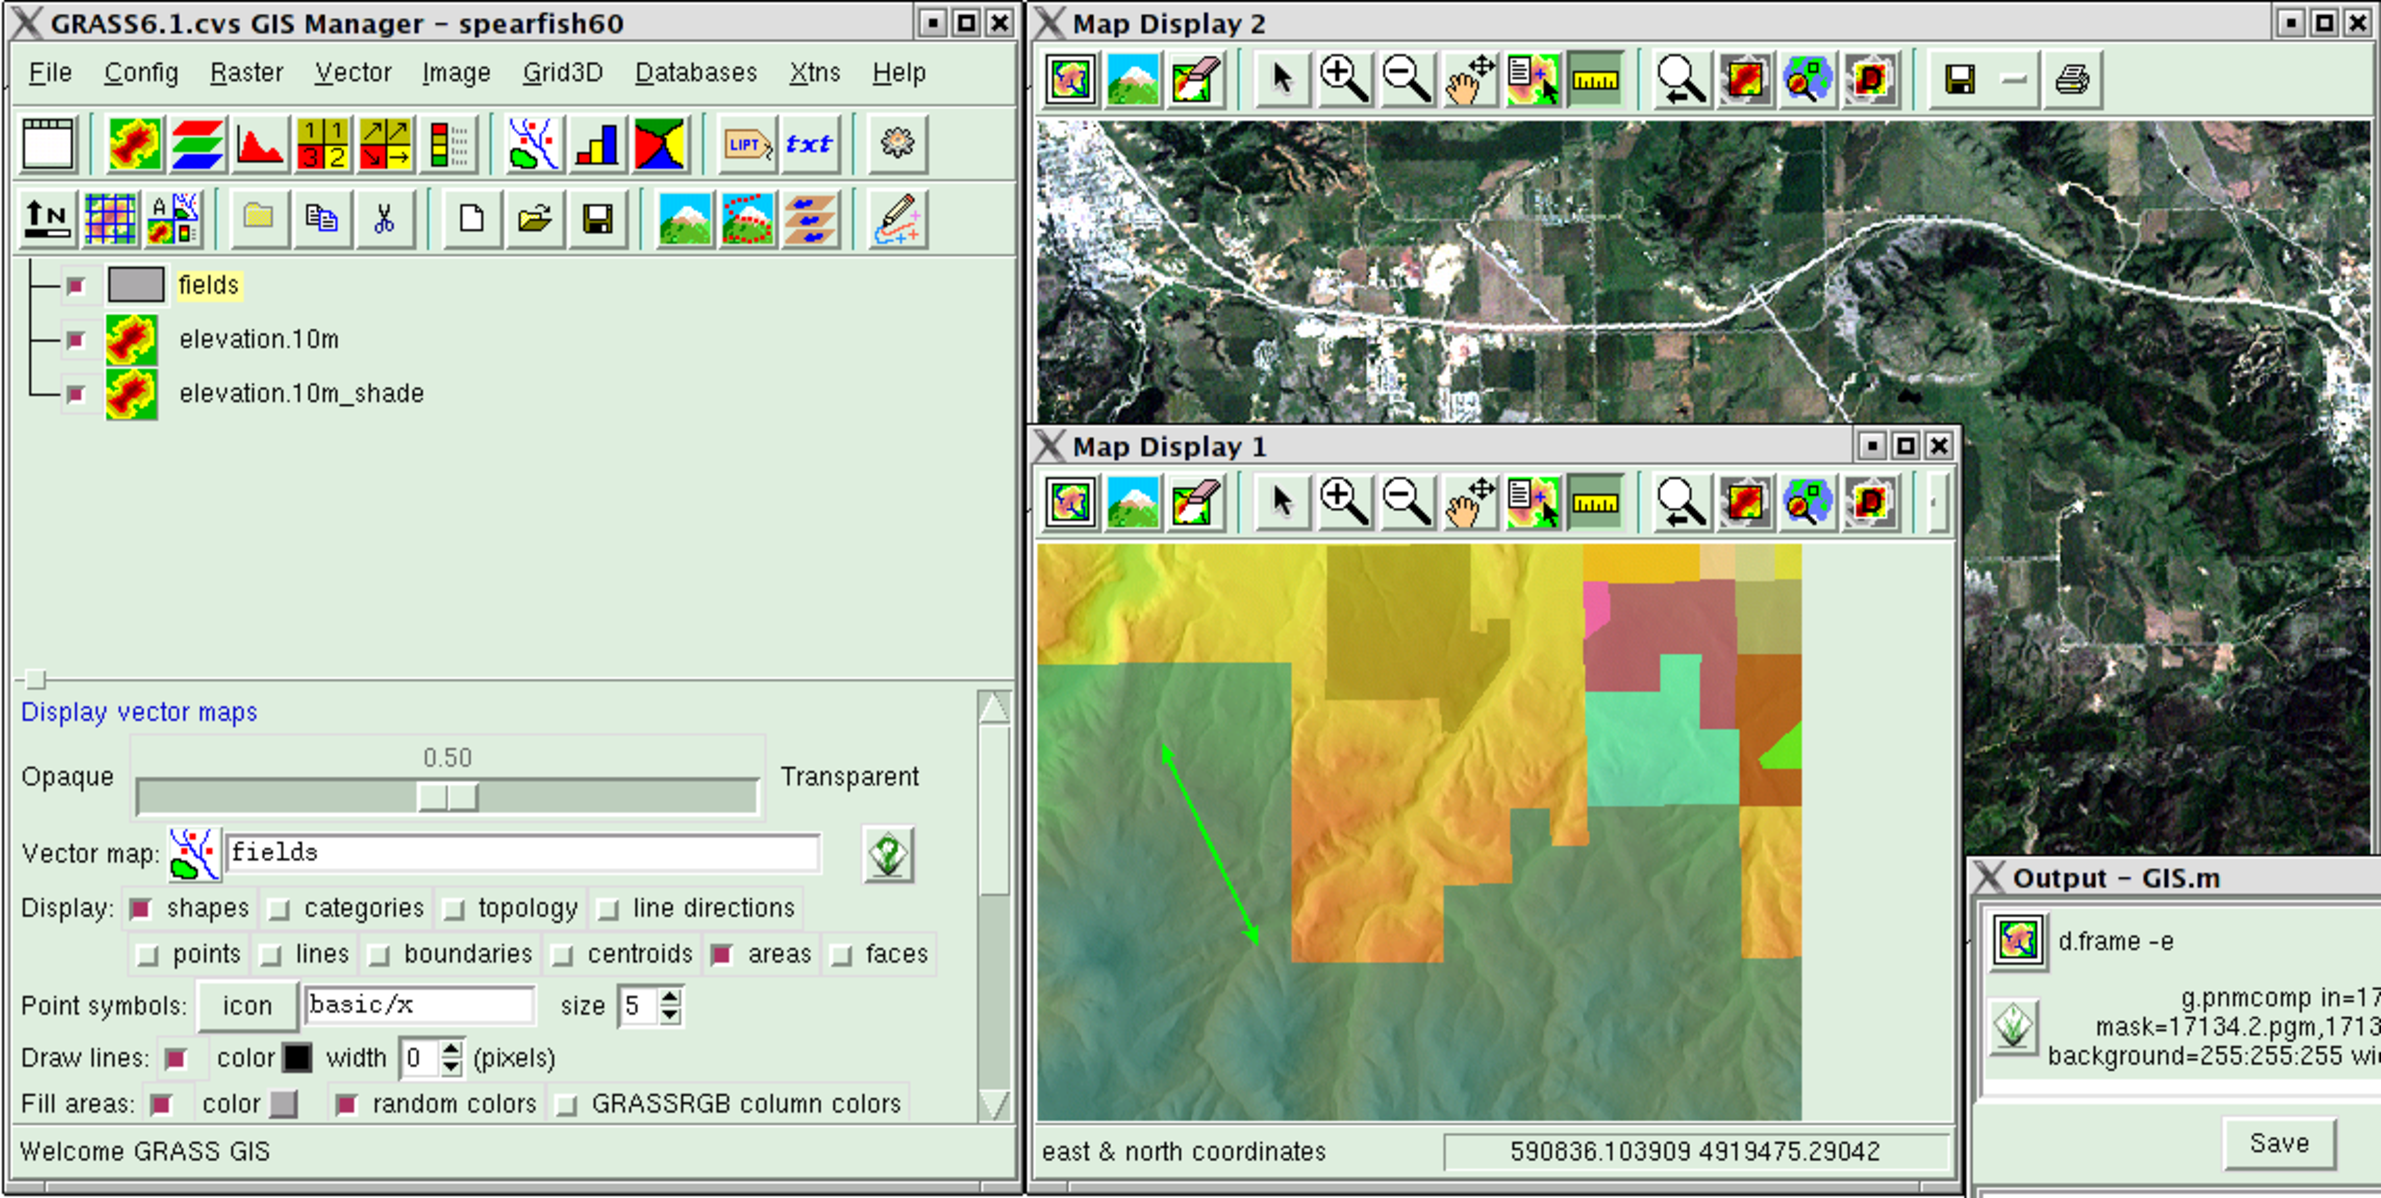
\includegraphics[width=0.70\textwidth]{grass-gis}
  \par}
  \caption{GRASS GIS interface.}
  \label{pic:grass}
\end{figure}

Originally GRASS GIS~\cite{grassgis} (see Figure~\ref{pic:grass}) was developed by US Army Construction Engineering
Research Laboratories and has a history of 30 years of the development. It is a powerful  and open-
source tool with large amount of capabilities. First, GRASS supports raster, voxel and vector
analysis and visualization. In addition to that, there is a toolbox for image processing, allowing
to apply variety of filters, adjust histograms and perform segmentation tasks. Finally, the program
supports numerous formats such as SQLite databases, PostgreSQL, mySQL, ODBC, CSV, satellite data,
UAV images.

The application of the GRASS GIS includes various fields such as archeology, cartography, geology,
geophysics and meteorology, although in our case it does not suit for the task. On of the  biggest
drawbacks is steep learning curve. The program requires extended knowledge from  the user in the
field of the geographical analysis and programming. The target audience are scientists and
engineers. Another  problem is complex installation and distribution process. On Mac OS X, the
installation  requires six dependent libraries. Moreover, the last version of the Mac OS X (10.11)
is not  supported.

\subsubsection{QGIS}

\begin{figure}[ht]
  {\par\centering
  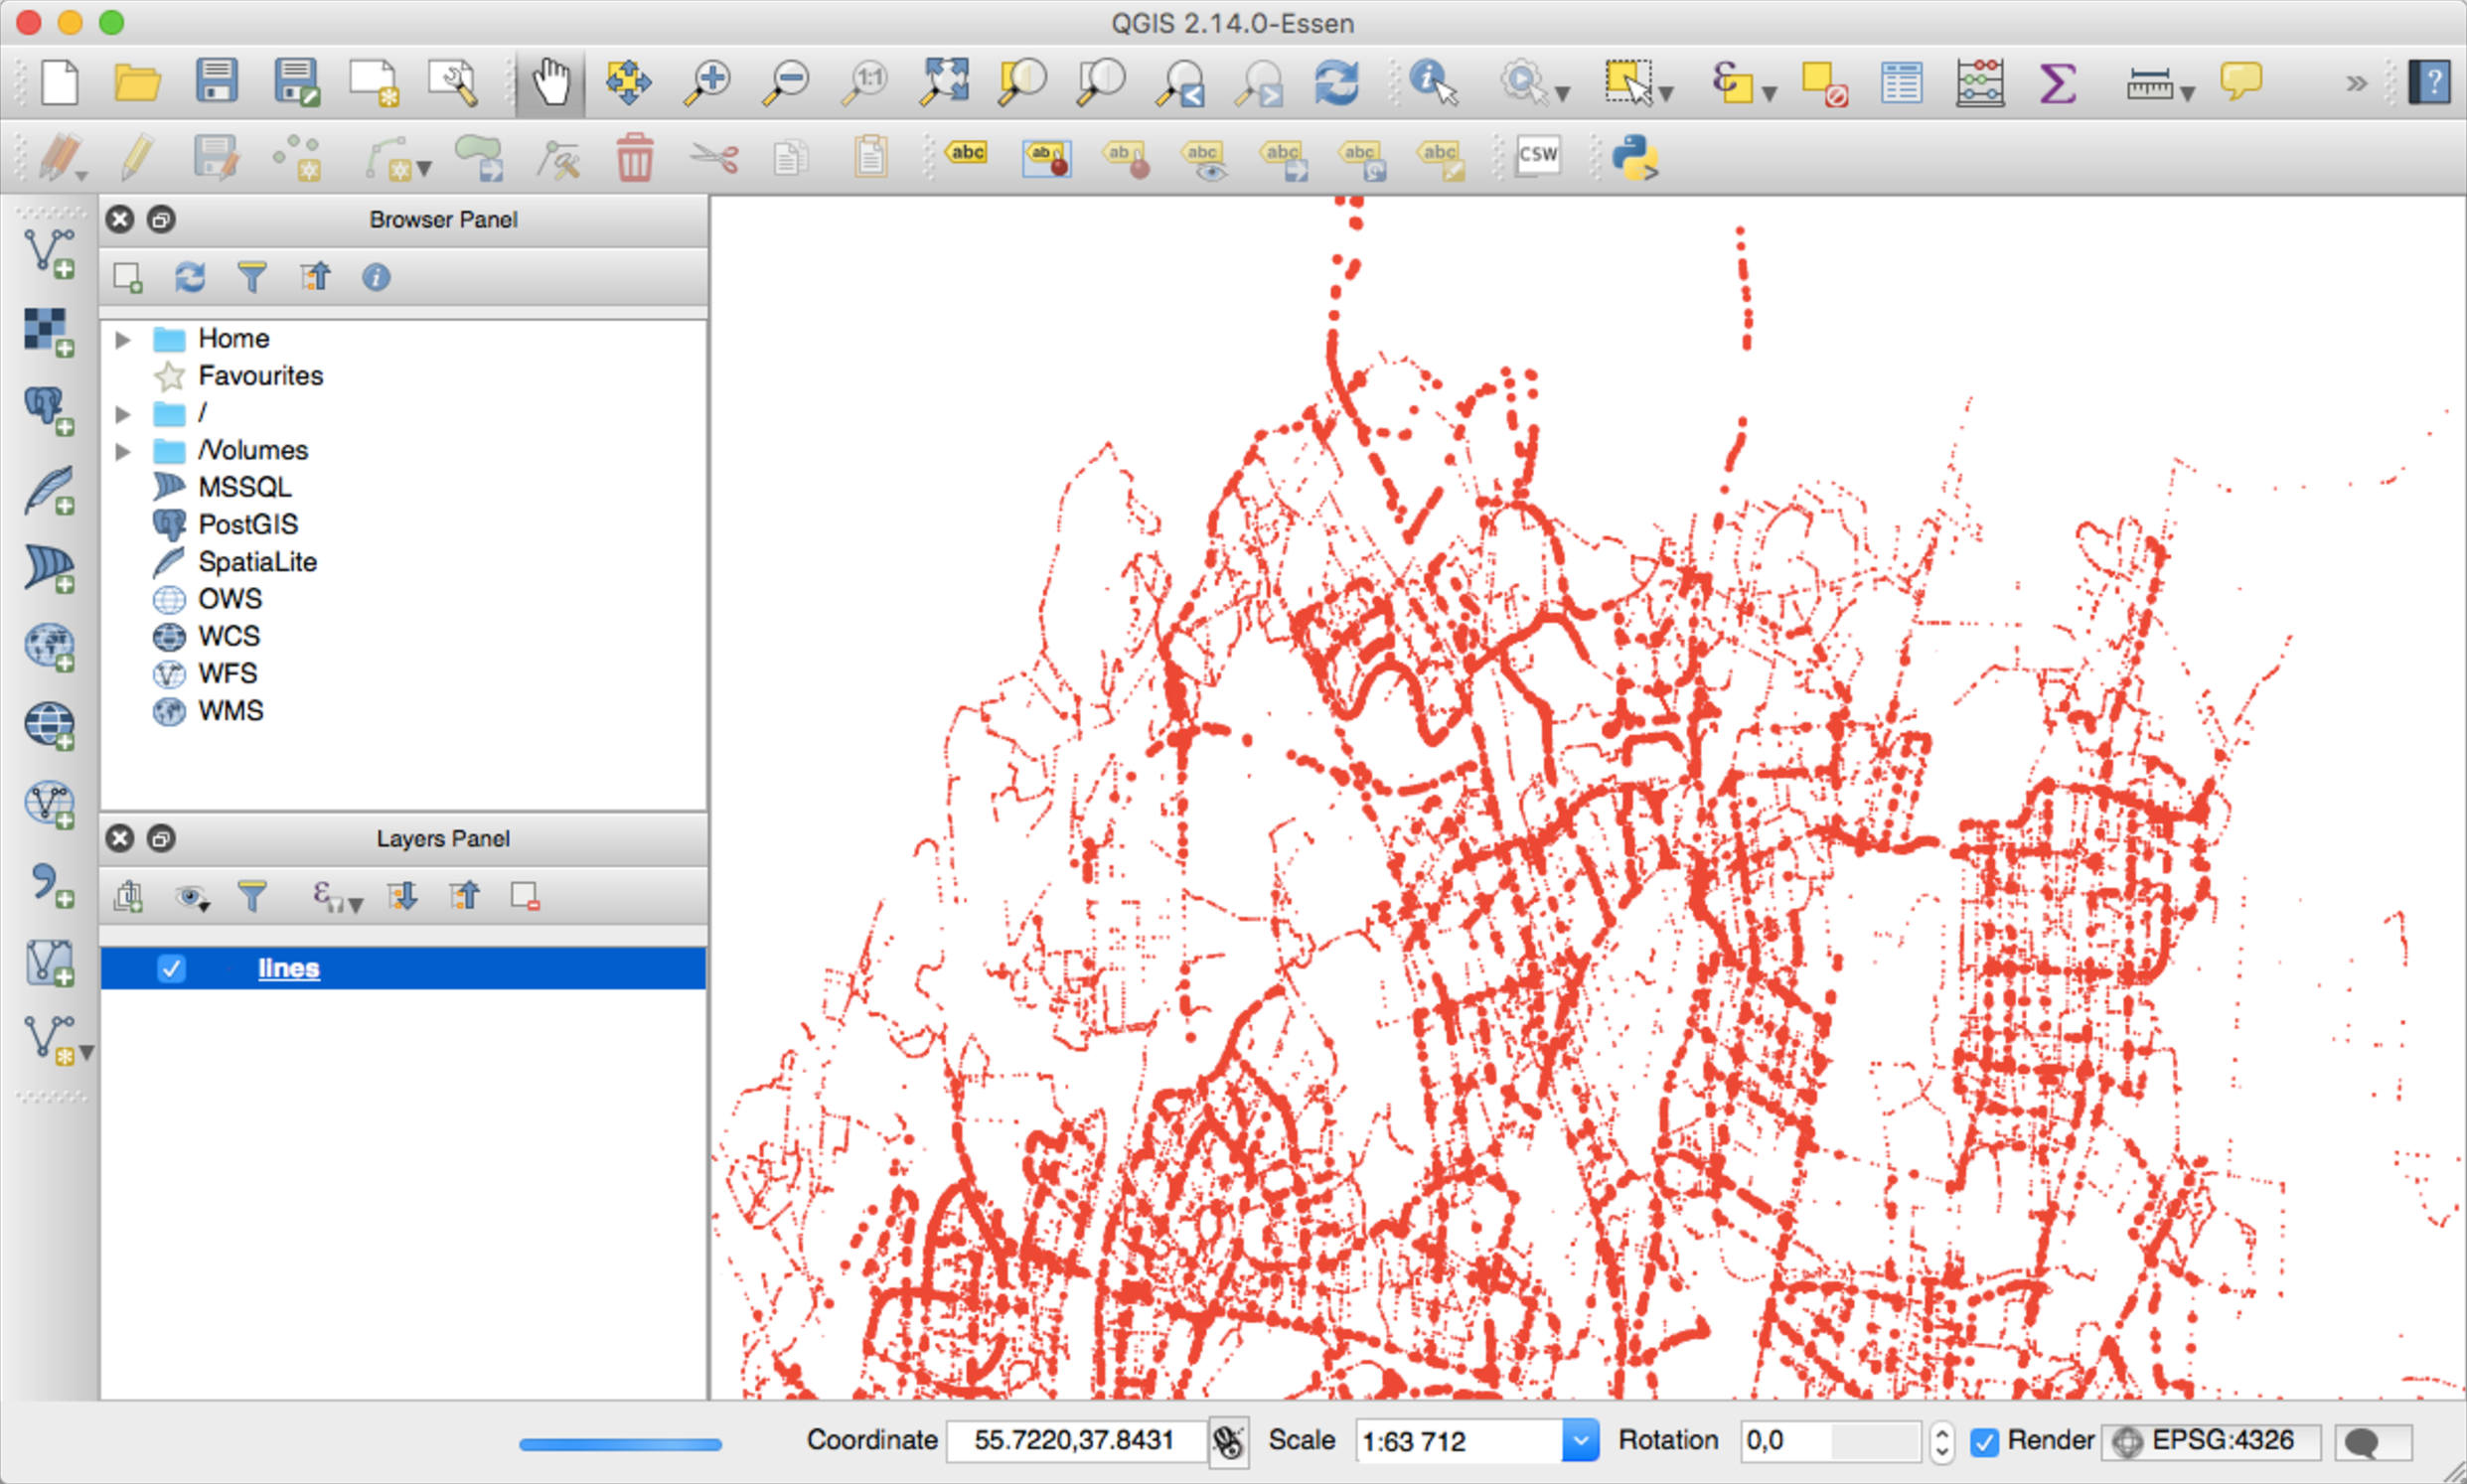
\includegraphics[width=0.70\textwidth]{qgis}
  \par}
  \caption{QGIS interface.}
  \label{pic:qgis}
\end{figure}

QGIS~\cite{qgis} is a free software for geographical data viewing, editing and analysis. The
software is licensed under GNU GPL. The development process started in 2002 with extensive use of
the Qt library. QGIS runs on multiple operating systems including Mac OS X, Linux and Windows. The
functionality of the QGIS can be extended via plug-ins written in Python.

Although QGIS lacks some features of the GRASS GIS, it has simpler UI (see example on
Figure~\ref{pic:qgis}) and does not have support of latest Mac OS X (10.11). Moreover, there are web
based implementations of the QGIS such as QGIS Server and QGIS Web Client. On the other hand, the
interface is still requires some programming and geographical background.

\subsubsection{CartoDB}

\begin{figure}[ht]
  {\par\centering
  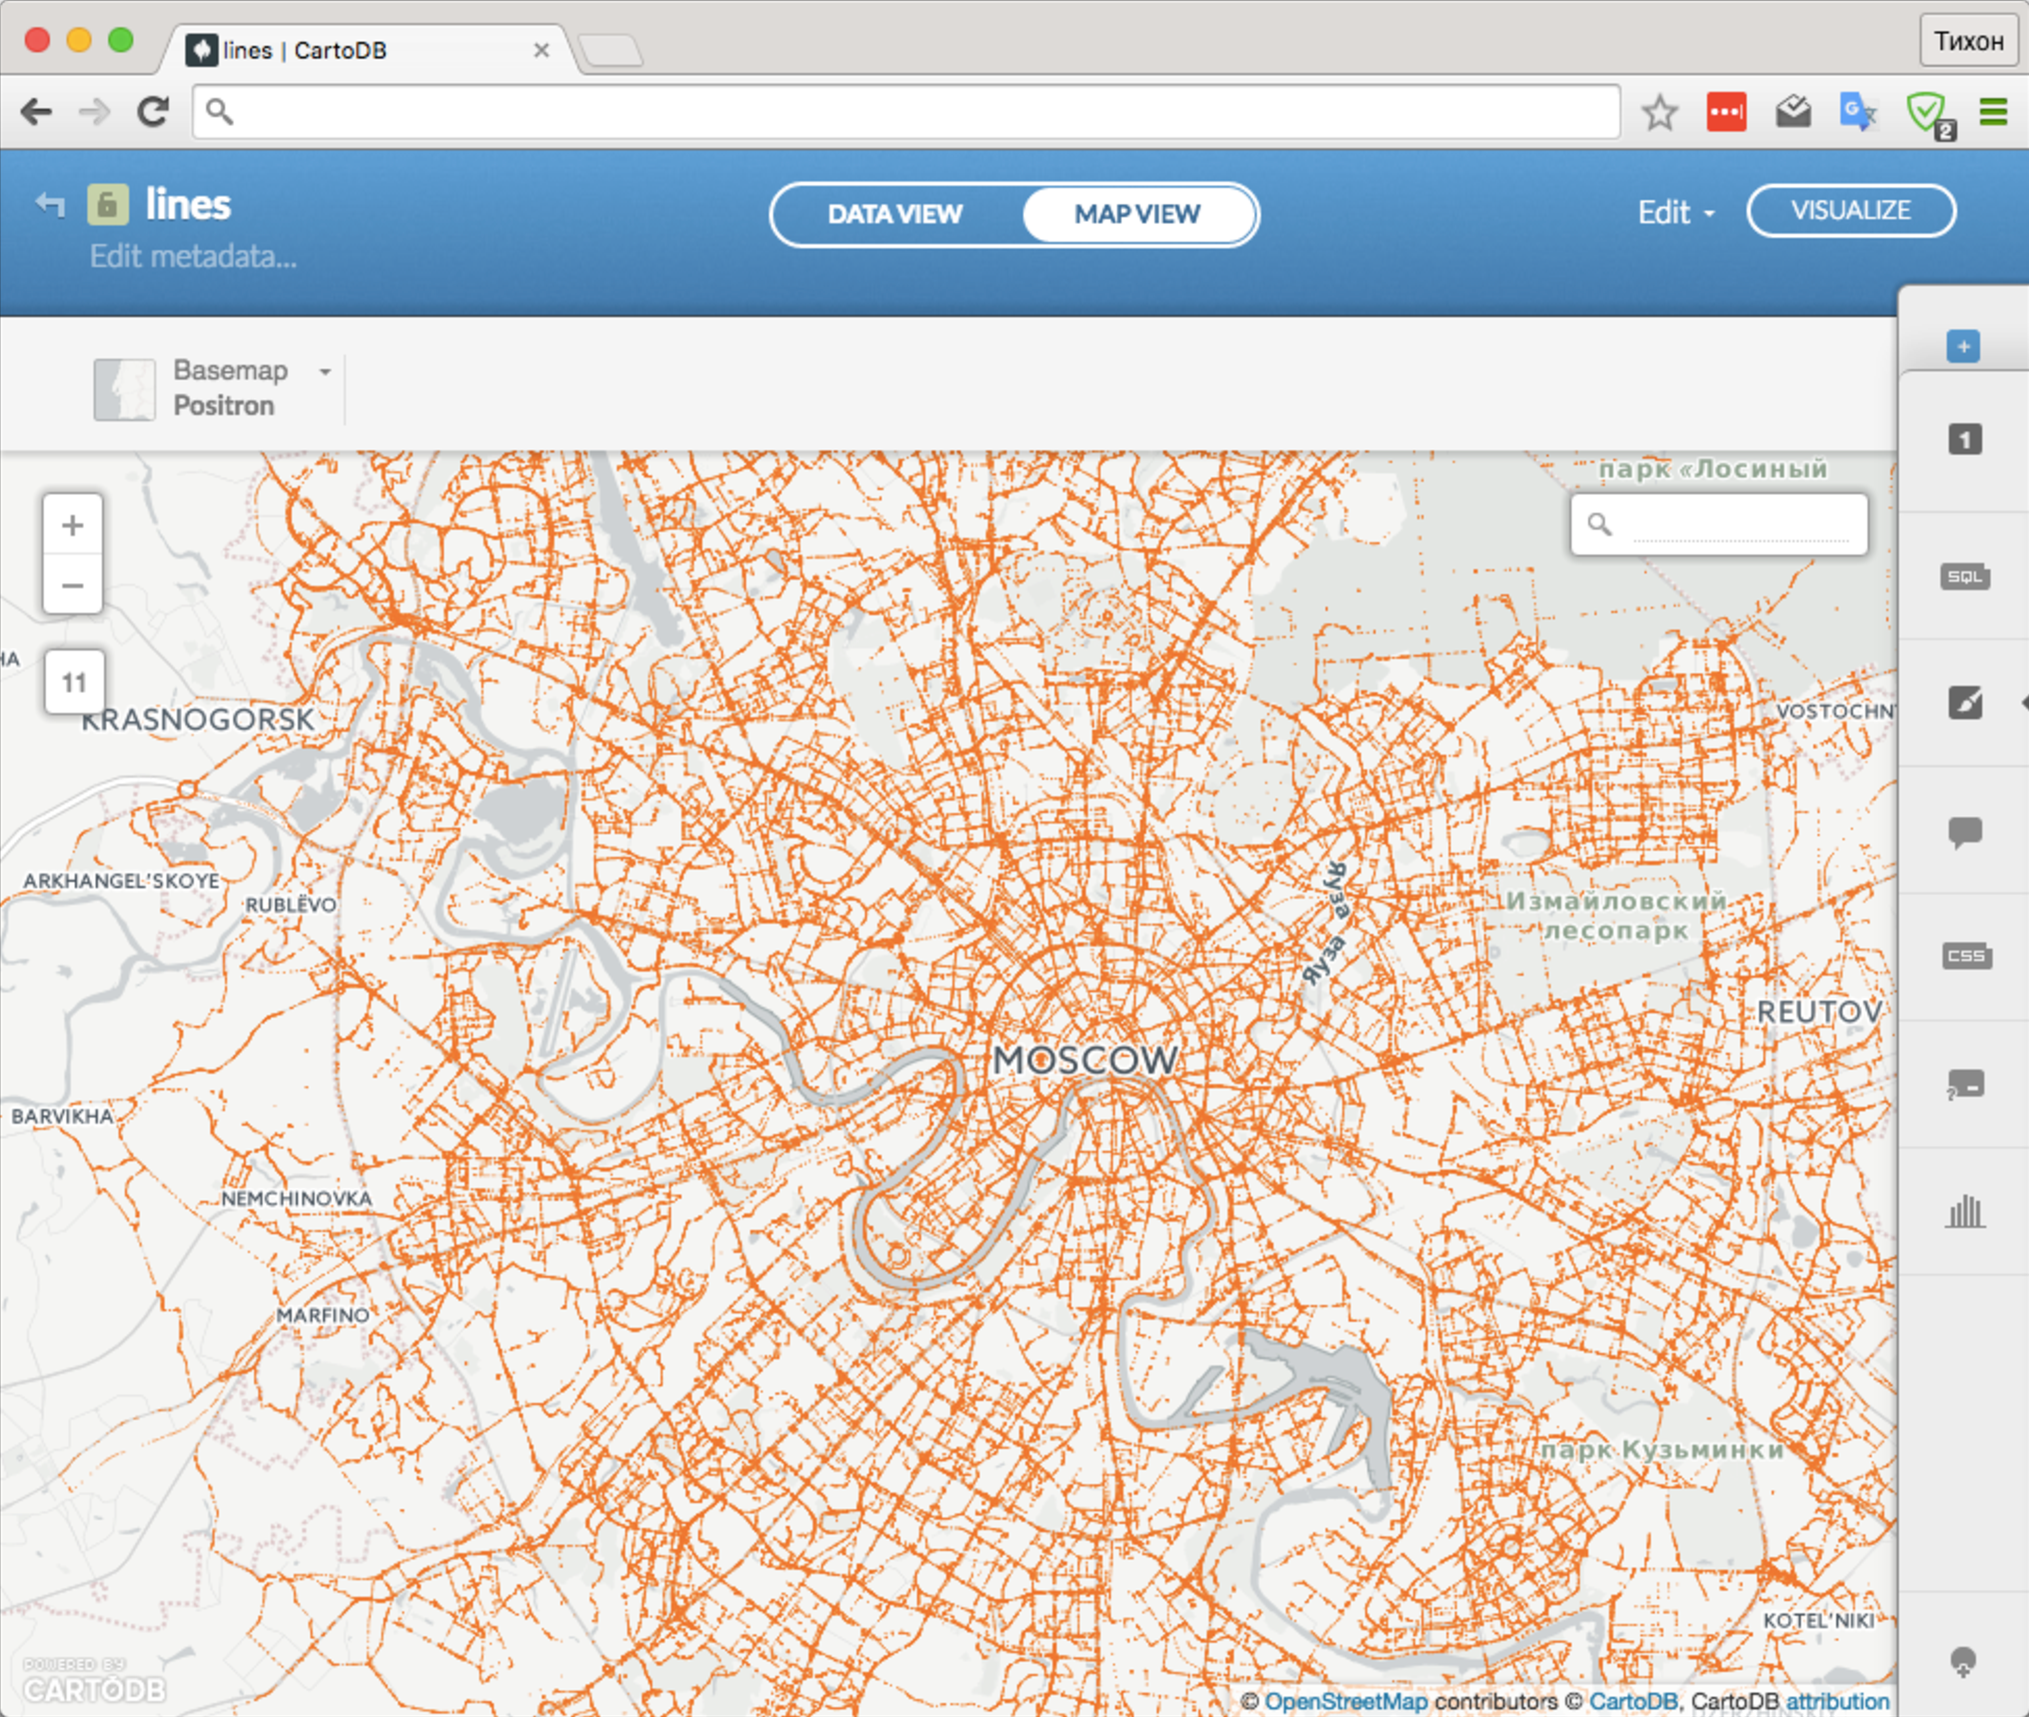
\includegraphics[width=0.70\textwidth]{cartodb}
  \par}
  \caption{CartoDB interface.}
  \label{pic:cartodb}
\end{figure}

CartoDB~\cite{cartodb} is a browser based proprietary solution for mapping and analysis, which
provides simplest interface (example on Figure~\ref{pic:cartodb})in comparison to GRASS GIS and
QGIS. Indeed, CartoDB is a great tool for creating interactive maps for the user without particular
background in the field. Another huge plus of the platform is simplicity of the distribution.
Basically anyone with access to the Internet and modern browser can view interactive map. However,
for our purpose the performance was not sufficient and basic filtering over the dataset was taking
up to 10 seconds.

\subsubsection{Summary}

Among all of the presented solutions, simple user interface and access with browser makes CartDB a
good candidate for the task. Yet, there is an issue with rendering performance which can hardly  be
solved. Second problem is the restrictions of the API making impossible to implement some of the
functionality. Finally, it should be underlined that CartoDB free plan does not support datasets
larger than 250 MB.

\subsection{Modern Web-based Maps}
In our application the choice of maps library should be made. In this section several
libraries for maps drawing are reviewed. The pluses and minuses of each of the
library are considered.

\begin{description}

  % Google
  \item[Google Maps Javascript API] -- on of the most popular libraries
    on the list~\cite{google:maps}. \\
    \underline{\smash{Pluses:}}
    \begin{itemize}
      \item Maps styling.
      \item Supports different localization options.
      \item The most detailed map across the world.
      \item StreetView.
      \item Support for mobile devices.
    \end{itemize}

    \underline{\smash{Minuses:}}
    \begin{itemize}
      \item Does not support vector tiles.
      \item Limited support for custom tiles.
      \item Free until exceeding 25,000 map loads per 24 hours for 90 consecutive days.
    \end{itemize}

  % Leaflet
  \item[Leaflet.js] -- lightweight mobile-friendly interactive maps
    library~\cite{leaflet}. \\
    \underline{\smash{Pluses:}}
    \begin{itemize}
      \item Small size -- only 33 KB of JavaScript code.
      \item Relatively simple API.
      \item Support for custom tile sources.
      \item Support for multilayer maps.
      \item Considerable amount of plug-ins.
      \item Free and open-source.
    \end{itemize}

    \underline{\smash{Minuses:}}
    \begin{itemize}
      \item Does not support vector tiles.
      \item Lack of Russian localization.
    \end{itemize}

  % Yandex Maps
  \item[Yandex Maps] -- best maps fidelity in Russia~\cite{yandex:maps}. \\
    \underline{\smash{Pluses:}}
    \begin{itemize}
      \item Highly detailed maps of Russia.
      \item Support of Russian localization.
      \item No restrictions for map views.
    \end{itemize}

    \underline{\smash{Minuses:}}
    \begin{itemize}
      \item Does not support vector tiles.
      \item Does not support map styles.
      \item Does not support custom tiles rendering.
      \item Proprietary.
    \end{itemize}

  % Mapbox GL JS
  \item[Mapbox GL JS] -- only library with whole vector tiles support~\cite{gh:mapboxgljs}. \\
    \underline{\smash{Pluses:}}
    \begin{itemize}
      \item Supports vector tiles.
      \item Supports real-time maps styles.
      \item Supports custom tile source.
      \item Based on Leaflet API.
      \item Open source.
    \end{itemize}

    \underline{\smash{Minuses:}}
    \begin{itemize}
      \item Standard tile source has limitations on views per month.
      \item Not fully detailed map of Russia.
      \item Lack of Russian localization.
    \end{itemize}
\end{description}

\subsection{Data Formats}

In the process of the development of transport accessibility analysis tool several
particular data formats were used. In this section utilized formats will be described.

\subsubsection{GeoJSON}

One of the most extensively used formats for encoding various types of geographical data is
GeoJSON which is actually a subset of JSON format~\cite{geojson:spec}. GeoJSON can store information
about such objects as Point, MultiPoint, Line, LineString, MultiLineString, Polygon. Geometric
objects which have some additional properties are stored as Feature objects. Moreover,
Features can be organized in feature collection. The example of the location which
represents center of the Moscow can be encoded as described on Listing~\ref{lst:geojson}.

\begin{lstlisting}[language=json, caption=GeoJSON data example.,
      label={lst:geojson}]
{
  "type": "Feature",
  "geometry": {
    "type": "Point",
    "coordinates": [37.61581, 55.74489]
  },
  "properties": {
    "name": "The Center of Moscow"
  }
}
\end{lstlisting}


The GeoJSON is text data format which results in larger size of the transfered data in comparison
with binary formats. Although, usually on the server it can be compressed using gzip~\cite{gzip}
which has native support in modern browsers. Compression results in dramatical size reduction up to
5 times in general case. However, it should be mentioned that archiving adds small overhead in
coding and decoding steps.

\subsubsection{Geobuf}

Geobuf is a compact data format for encoding geographical data. The format is based on Protocol
Buffers -- language-neutral mechanism developed by Google for serializing structured
data~\cite{protobuf}. Geobuf allows losslessly transformation of the GeoJSON data into protocol
buffers. There are several important advantages like faster compression in comparison to even native
JSON \texttt{parse} and \texttt{stringify} methods. Another valuable attribute of this format is
compact size, which is 8 times smaller than raw GeoJSON and 2 times smaller than GeoJSON after
applying gzip compression. The comparison of GeoJSON and Geobuf in terms size is presented on
Table~\ref{tab:geobuf}.

\begin{table}[ht]
  \renewcommand{\arraystretch}{1.5}
  \centering
  \begin{tabular}{l l l}
    \hline
    & \textbf{normal} & \textbf{gzipped} \\
    \hline
    us-zips.json & 101.85 MB & 26.67 MB \\
    % \hline
    us-zips.pbf & 12.24 MB & 10.48 MB \\
    % \hline
    idaho.json & 10.92 MB & 2.57 MB \\
    % \hline
    idaho.pbf & 1.37 MB & 1.17 MB \\
    \hline
  \end{tabular}

  \caption{Sample compression sizes~\cite{geobuf}.}
  \label{tab:geobuf}
\end{table}

\subsubsection{MBTiles}

Web maps may contain million of tiles, hence there is clearly a problem in storing and managing such
enormous amount of data. To overcome the problem of handling so many tiles data Mapbox team has
developed open-source data format for storing tiles in a single SQLite data base.

SQLite is claimed to be ideal for the purpose of storing tiles since it is available on all of the
platforms including mobile devices. Each \texttt{.sqlite} data base is self-contained and does not
require any special setup, which results in high portability.

Another great feature of the MBTiles format is the ability to effectively store duplicate tiles. As
an example the tile located in the middle of the ocean can be considered (see
Figure~\ref{pic:water-tile}). It is clear that there is considerable amount of tiles containing
solid blue color. Taking in account all of the zoom levels it can lead to millions of the
duplicates. However, MBTiles can reference thousands of tiles to the same image without
the need for loading all look-alike pictures.

\begin{figure}[ht]
  {\par\centering
  
\includegraphics[width=0.20\textwidth]{water-tile}
  \par}
  \caption{Example of the tile duplicate.}
  \label{pic:water-tile}
\end{figure}

Important to note that MBTiles may be used to store both image-based tiles encoded in PNG or
vector tiles encoded in Protocol Buffers. This is a crucial detail since vector tiles
allow real-time styling and provide smoother zooming.







